% #################################################################################
%
% Template LaTeX pour le CFA2025 Paris
% Les lignes 8 à 113 déterminent le style utilisé pour les articles du CFA2025
% Les auteurs sont invités à modifier le contenu à partir de la ligne 113.
%
% #################################################################################
\documentclass[a4paper,final,10pt]{article}
% Décommenter une des trois lignes suivantes pour indiquer le codage du fichier tex
%\usepackage[latin1]{inputenc}
%\usepackage[ansinew]{inputenc}
\usepackage[utf8]{inputenc}

\usepackage[T1]{fontenc}
\usepackage[french]{babel} % option french
\usepackage{amsmath}
\usepackage{txfonts}
\usepackage{enumitem}
\usepackage{geometry} % used to set margins
\usepackage{fancyhdr, eso-pic}
%\usepackage[]{authblk}
%\renewcommand\Authand{ et }\renewcommand\Authand{ et }
\usepackage{xcolor,graphicx} % used to insert the figure
\usepackage{hyperref}
\usepackage{multirow}   % pour les cellules multilignes dans les tableaux
\usepackage{listings}   % pour insérer des extraits de code

% En cas d'erreur de compilation indiquant \qty ou \sisetup
% commentez les 10 lignes qui suivent et n'utilisez pas ces macros
\usepackage{siunitx}    % pour écrire des unités physiques
\makeatletter
    \ifdefined\qty
      % Une version récente de siunitx est visiblement disponible
      \sisetup{uncertainty-mode=separate, separate-uncertainty-units=repeat,
               input-open-uncertainty=[,input-close-uncertainty=]}
    \else
      % Sinon, ersatz de contournement qui ne gère pas les incertitudes...
      \newcommand{\qty}[1]{\SI{#1}}
      \sisetup{separate-uncertainty, range-units=single}
    \fi
\makeatother

\hyphenpenalty=10000
\setlength{\emergencystretch}{3em}
\hypersetup{colorlinks=true, linkcolor=blue, filecolor=red, urlcolor=red, citecolor=teal}
\geometry{hmargin=1.5cm, vmargin=2.5cm}
\setlength{\columnsep}{1cm}
\setlength{\parindent}{0.5cm}
\setlength{\parskip}{0em}
\setlength{\intextsep}{12pt}
\setlength{\abovecaptionskip}{12pt}
\setlength{\belowcaptionskip}{5pt}
\setlist[itemize,1]{label=\textbullet, partopsep=0pt, itemsep=3pt, topsep=6pt, parsep=0pt}
\renewcommand\frenchtablename{Tableau}
\lstnewenvironment{code}[1][]{\lstset{#1}}{} % Add/update settings locally
\lstset{frame=leftline, basicstyle=\ttfamily\small, language=Python, %
    showspaces=false, showstringspaces=false}  % Global options

% Style fancy
\pagestyle{fancy}\fancyhf{}
\lhead{17\textsuperscript{e } Congrès Français d'Acoustique}
\rhead{27-30 avril 2025, Paris}
% \cfoot{\thepage}

\makeatletter
\def\ifdraft{\ifdim\overfullrule>\z@
  \expandafter\@firstoftwo\else\expandafter\@secondoftwo\fi}
\renewcommand*{\maketitle}{
   \AddToShipoutPicture*{
    \put(0,0){\parbox[b][0.4663\paperheight]{\paperwidth}{ % 0.4663 ~ 0.5*(817/876)
        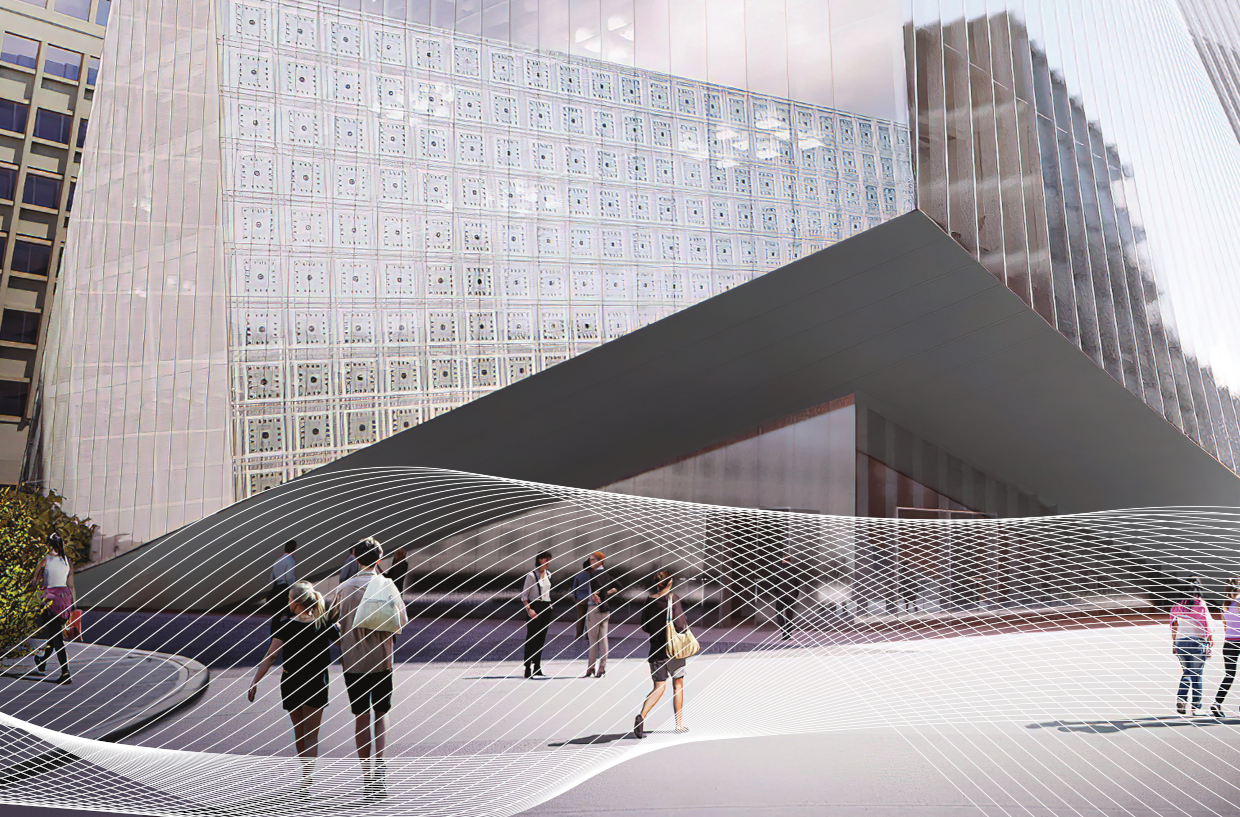
\includegraphics[width=\paperwidth,height=0.4663\paperheight]{FondPageGarde.jpg}
    }}}
    \begin{titlepage}
    \thispagestyle{empty}
    \centering
    \setlength{\fboxrule}{2pt}
    \parbox[c][.99\textheight][t]{.99\textwidth}{
    \begin{center}
    
\includegraphics[width=55mm,keepaspectratio=true]{LogoCFA2025.pdf}\\[.5cm]
    {\Large 17\textsuperscript{e} Congrès Français d'Acoustique\unskip\strut\par}
    {\Large 27-30 avril 2025, Paris\unskip\strut\par}
    \vspace{1cm}
    {\LARGE \@title \par}%
    \vskip 3em%
    {\large
    \lineskip .75em%
      \begin{tabular}[t]{c}%
        \@author
      \end{tabular}\par}
    \end{center}}%
  \end{titlepage}
}
\renewcommand{\section}{\@startsection{section}{1}{0pt}{21pt}{10pt}{\Large\bfseries}}
\renewcommand{\subsection}{\@startsection{subsection}{2}{0pt}{0pt}{5pt}{\large\bfseries}}
\makeatother

\newcommand{\resume}[1]{%
\twocolumn[
  \begin{list}{}{%
    \setlength{\topsep}{0pt}%
    \setlength{\leftmargin}{1cm}%
    \setlength{\rightmargin}{1cm}%
    \setlength{\listparindent}{\parindent}%
    \setlength{\itemindent}{\parindent}%
    \setlength{\parsep}{\parskip}}%
    \item #1
  \end{list}\vspace{24pt}]
  }
\newenvironment{listing}{\begin{footnotesize}\begin{verbatim}}{\end{verbatim}\end{footnotesize}}


%%%%%%%%%%%%%%%%%%%%%%%%%%%%%%%%%%%%%%%%%%%%%%%%%%%%%%%%%%%%%%%%%%%%%%%%%%%%%%%%%%%%%%%
% En principe ICI commence la partie du fichier à éditer par les auteurs

\title{Modèle \LaTeX ~d'article 6 pages pour le CFA2025}
%%%% Begin - AUTEURS : VERSION DE BASE sans  \usepackage{authblk}
\author{
J.~Suispremierauteur $^{a}$,~ 
E.~Moiledeuxieme $^{b}$~
et~P.~Uiletrois $^{a,b}$
\\
$^{a}$ {\small Sorbonne Université, CNRS, Institut Jean Le Rond d'Alembert, F-75005 Paris, France} 
\\ 
$^{b}$ {\small Secrétariat de la SFA, 44 rue Pasquier, F-75008 Paris, France}
\and 
}
%%% End - AUTEURS : VERSION DE BASE sans  \usepackage{authblk}
%\author[a]{J.~Suispremierauteur}
%\author[b]{~E.~Moiledeuxieme}
%\author[a,b]{et~P.~Uiletrois}
%\affil[a]{Sorbonne Université, CNRS, Institut Jean Le Rond d'Alembert, F-75005 Paris, France}
%\affil[c]{Secrétariat de la SFA, 44 rue Pasquier, F-75008 Paris, France}
\date{}  %no date


\begin{document}
\maketitle %  Commenter pour supprimer la page de garde

\resume{Ce paragraphe contient le \textbf{résumé} de votre manuscrit au CFA~2025-Paris. De même que pour l'édition 2022 du CFA à Marseille, les articles obtenus avec les modèles \LaTeX~, ODT et DOCX comportent une page de garde (qui ne sera donc pas ajoutée par le serveur). 
Le résumé figure en tête de seconde page, conformément au présent document. Il est en simple colonne (style \textbf{Abstract} dans LibreOffice et Word), justifié, avec une taille de caractères de 10~pt, 
et une indentation de 1~cm des deux côtés. Il ne doit pas contenir de références, figures, équations, ou symboles mathématiques. Il doit contenir entre 120 et 300 mots, et être suivi d'un espace vertical de 24~pt. Il est recommandé de reprendre ici le résumé accepté 
(avec éventuellement des corrections mineures). Toute modification des titre, auteurs, affiliations et résumé devra être également reportée sur la plateforme des résumés. Toute modification faite après le \textbf{15 mars 2025} ne pourra être prise en compte dans les actes et le programme.}

\section{Introduction}
\par Veuillez lire les instructions suivantes avant de commencer la rédaction de votre manuscrit, 
ce qui assurera une homogénéité de style dans les actes du congrès.
\par Votre manuscrit sera soumis au format PDF, seul format accepté par le serveur pour cette édition du CFA. Un exemple de manuscrit final est disponible à l'adresse :
\begin{center}
\href{https://cfa2025.fr/pdfs/cfa2025-article-LaTeX-reference.pdf}{https://cfa2025.fr/pdfs/cfa2025-article-LaTeX-reference.pdf}
\end{center}
\par \textbf{Votre manuscrit ne doit pas excéder 7~pages, page de titre \underline{incluse}, 
et la taille du fichier PDF final ne doit pas excéder 4~MB.}

\section{Soumission du manuscrit}
\par La date limite pour le dépôt du manuscrit est le \textbf{\underline{15 mars 2025}}. 
Aucune extension n'est prévue à ce jour. Ce dépôt se fait sur le site du congrès exclusivement :
\begin{center}
\href{https://conforg.fr/bin/usrlogin\_cfa2025}{https://conforg.fr/bin/usrlogin\_cfa2025}
\end{center}

\par Après soumission du manuscrit, vous recevrez une confirmation par e-mail contenant le fichier PDF final.
Vérifiez ce fichier aussi vite que possible de telle sorte qu'un nouveau manuscrit puisse être re-déposé avant la date limite en cas de besoin.
\par Si vous ne recevez pas de confirmation dans les 24~h suivant votre soumission, pensez à vérifier qu'il n'a pas été classé comme pourriel, puis contactez-nous par email à l'adresse:
\begin{center}
\href{mailto:soumissions-cfa2025@sfa.asso.fr}{soumissions-cfa2025@sfa.asso.fr}
\end{center}
\par Merci d'indiquer dans votre mail les références données par le serveur à la fin du processus de soumission (ou à défaut, si vous n’en disposez pas, le numéro du résumé).

\section{Format du manuscrit}

\subsection{Mise en page}
\par Le manuscrit est au format A4 (210~mm x 297~mm).
Les marges latérales et verticales doivent être mises à 1.5~cm.
À l'exception du résumé, le texte est disposé en deux colonnes de 8.5~cm séparées par un espace de 1~cm. 
Des exceptions sont possibles (pour l'insertion d'équations longues ou de grosses figures).
\par La fonte de caractères utilisée est de type {\bf Times New Roman}, et les tailles des caractères pour les paragraphes et les différents titres de section sont spécifiées dans le Tableau~\ref{tab:format}.

\begin{table}[h]
\center
\caption{Styles de paragraphes.} % Titre du tableau avant le tableau
\label{tab:format}
\begin{tabular}{|p{18mm}|r|r|r|c|}
\hline
\multirow{2}{18mm}{\bf Style} & \multirow{2}{8mm}{\bf Taille carac.} %
& \multicolumn{2}{|c|}{\bf Espacements} & \multirow{2}{17mm}{\bf Alignement} \\
\cline{3-4} & & dessus & dessous & \\ \hline\hline
Abstract & 10~pt & 0~pt & 24~pt & Justifié \\ \hline
Text Body & 10~pt & 0~pt & 0~pt & Justifié \\ \hline
Heading 1 & 14.4~pt & 21~pt & 10~pt & Gauche \\ \hline
Heading 2 & 12~pt & 10~pt & 5~pt & Gauche \\ \hline
Appendix & 14.4~pt & 21~pt & 12~pt & Gauche \\ \hline
Bibliography & 9~pt & 6~pt & 6~pt & Justifié \\ \hline
\end{tabular}
\end{table}


\subsection{Format des paragraphes}
\par Le texte de tous les paragraphes doit être justifié, avec des indentations de 0.5~cm. 
Il n'y a pas d'espaces verticaux entre les paragraphes. Une taille de caractères de 10~pt 
doit être utilisée pour le corps du texte, dans tout le document (style \textbf{Text Body} 
dans LibreOffice et MS Word).


\subsection{Sections et sous-sections}
\par Ces deux niveaux d'entêtes ne sont pas indentés.
L'espace vertical avant et après ces entêtes est indiqué dans le Tableau~\ref{tab:format}. 
Les utilisateurs de LibreOffice et MS Word doivent choisir le 
style \textbf{Heading 1} pour la section de premier niveau et \textbf{Heading 2} pour 
le second niveau et éviter d’ajouter des sections de niveau inférieur.

\subsection{Tableaux}
Les tableaux doivent être centrés dans la colonne (ou dans la page si leur taille 
est trop importante). Ils doivent être séparés du texte par un espace de 12~pt. 
La légende (style \textbf{Caption/Table}) doit être placée au-dessus des tableaux. 
Ceci est une référence au Tableau~\ref{tab:format}.

\subsection{Figures}
\par Les figures doivent être centrées dans la colonne (ou éventuellement dans la page). 
Elles sont suivies par une légende (style \textbf{Caption/Figure}), cf. Figure~\ref{fig:logo_cfa2025}. 
Les figures sont séparées du texte par un espace de 12~pt.
\par Préférez les images dans un format vectoriel (PDF). À défaut, utilisez si possible
une résolution d'au moins 300~dpi pour que les figures soient lisibles.
\begin{figure}[h]
\centering

\includegraphics[width=65mm,keepaspectratio=true]{LogoCFA2025.pdf}
\caption{Logo du CFA2025-Paris. La légende est séparée de la figure par un 
espace de 12~pt et du texte par un espace de 12~pt.}
\label{fig:logo_cfa2025}
\end{figure}

\subsection{Listes}
\par Les listes doivent être séparées du texte par un espace de 6~pt (style \textbf{List1}). 
Les éléments de la liste débutent avec une puce et sont indentés de 0.5~cm par rapport à la marge gauche.
Un espace vertical de 3~pt est laissé entre les éléments.
\begin{itemize}
\item Premier élément,
\item Deuxième élément,
\item Troisième élément.
\end{itemize}


\subsection{Listings}
\par Les listings de programme (style \textbf{Listing}) doivent être séparés du texte par un espace 
vertical de 12~pt et être écrits dans une fonte de caractères \textbf{Courier New}, avec une taille de caractères de 8~pt.

\begin{code}
    from datetime import date
    a = date(2025, 4, 27)
    print(f'Rendez-vous au CFA{a.year}'
          f'le {a.strftime("%d/%m/%y")} !')
\end{code}

\subsection{\'{E}quations}
\par Les équations sont centrées (style \textbf{Equation}) et numérotées,
avec le numéro aligné à droite:
\begin{equation}
\begin{split}
x & =\frac{1}{a-b}\\
%  & = \SI{50.0\pm 0.1}{\meter} % siunitx v2
  & = \qty{50.4\pm 1.2}{\meter} % siunitx v3
\end{split}
\label{eq:limit}
\end{equation}

Ceci est une référence à l'Eq.~(\ref{eq:limit}). Utiliser une version récente du paquet \emph{siunitx} (v3) pour gérer les unités et les incertitudes !

\section{Références}
\par La liste des références doit apparaître en fin de document et l'entête ne 
doit pas comporter de numéro (style \textbf{Appendix}).
\par Laissez un espace de 6~pt entre les différentes entrées  (style \textbf{Bibliography}), celles-ci étant en taille 9~pt. Les citations dans le texte se font avec 
des crochets comme ceci \cite{refmyers}. Les citations multiples sont séparées par 
une virgule \cite{refmyers,refwhitham}.

\section{Conclusion}
Merci pour votre participation au CFA2025 à Paris !

\section*{Remerciements}
L'entête de la section des remerciements n'est pas indenté (syle \textbf{Appendix}), n'est pas numéroté et doit apparaître juste avant la section des références.

\small
\begin{thebibliography}{10}
\bibitem{refmyers} M.~K.~Myers, On the acoustic boundary condition in the presence of flow, \emph{Journal of Sound and Vibration} \textbf{71}, 429-434 (1980).
\bibitem{refwhitham} G.~B.~Whitham, \emph{Linear and nonlinear waves}, John Wiley \& Sons, New York (1974).
\end{thebibliography}

\end{document}


